\title{The A.I. Craft Project}
\author{
	Ray Shulang Lei\\
	aicraft.com\\
	ray.lei@uregina.ca
}
\date{\today}

\documentclass[12pt]{article}
\setlength{\parindent}{0in}
\usepackage{graphicx}
\usepackage{mathtools}
\usepackage{amsthm}
\usepackage{parskip}
\usepackage{hyperref}

\begin{document}
\maketitle

\begin{abstract}
Gamify Learning has recently gained popularity and believed to be effective for education purpose. Today’s economic has evolved to be ``developer-centric"\cite{venkatesh2011}. While we have many games to practice various skills in a fun way, there has not been too much efforts made for development skills.\\ 

There is a recently made popular practice called ``livecoding", where programmers perform art using their programming skills in real-time to interactively improvise their works on the fly.\\ 

A.I. Craft is a web based multi-player artificial intelligence combating game driven by livecoding competition between players. Players provide their code in real-time to control their A.I.s, in order to beat the opposite A.I.s. 
\end{abstract}

\section{Introduction}
Project A.I. Craft is the development of a livecoding A.I. combating game. According to wikipedia, livecoding can also be referred to as improvised interactive programming. Players use their programming skills to improvise their code in real time to control their A.I.s, in order to beat the opposite players. The idea is inspired by the JAVA Robocode\cite{robocode01} project. The main purpose is to ``gamify" the never-ending learning process for programming. To understand what ``gamify" means, here is the definition from wikipedia: ``Gamification is the use of game design techniques and mechanics to solve problems and engage audiences."\\

Not until recently, the dynamic programming languages have envolved to be fast and effecient enough for livecoding practice. With some new technologies I am going to introduce later ( HTML5, NodeJS ), javascript, is treading to be the unified programming language for the web. Powering by the Google's V8 engine, javascript has been use for livecoding in audio and visual arts at last year's Google IO conference openning show. A.I. craft is aimming to take the livecoding practice further into the video game world, seeing that the current technologies is mature enough.\\

\section{Rationale}

\subsection{Motivation}
In Noah Falstein's article ``Natural Funativity"\cite{noah2004}, he described three types of hunters in a hunter-gatherer society. After three hunters have got enough haunch of antelope, enough to feed his family for a few days:\\
Aagh - goes right back out to track down a deer he saw earlier;\\
Bohg - passes his time by kicking back and catching nothing more challenging than some rays;\\
Cragh - plays hunting games at home. ``Like Aagh, he is building survival skills - but does so it in the safe confines of home. Like Bohg, he stays safe - but also stays fit and slightly improves his chances for success in the next hunt. "\\

Noah Falstein concluded that ``Over hundreds of thousands of generations, those genes that Cragh carries are more likely to spread, and the activities - including games - can also be passed on through word of mouth in the tribe from generation to generation."\\

According to Venkatesh's article ``The Rise of Developeronomics"\cite{venkatesh2011} on Forbes, our society now is a developer-centric economy. He further argues that there are only two kinds of people matters: developers, and people who controls developers. Assuming our society is developer driven, I can conclude that the developers are as important as hunters in a hunter-gatherer society. What Aagh, Bohg and Cragh would be like in today's society? After developers finishes their work before the deadline, there would be three types of behaviors:\\
Aagh - goes right back out to code for more income, whether it is a contract job or freelancing;\\
Bohg - will be chilling out, get more sleep, let the brain rest;\\
Cragh - plays games at home to sharpen his development skills.\\ 

Now, let us think about what kinds of games Cragh can use to improve his development skills. First person shooters? It only makes a better hunter. Strategy games and others? Maybe, but they are still not exactly related to coding. Thus we need a new genre of games: coding games.\\

\subsection{Robocode}
Robocode is a educational coding game. Players write programs that controls a miniature tank that fights other identically-built (but differently programmed) tanks in an arena. Tanks can move, shoot at each other, scan for each other, and hit the walls (or other robots) if they aren't careful. When I first start looking for coding games, Rococode is the closest to what I am looking for.\\

Project A.I. craft is inspired by the Robocode, and thus originated from it. Let us look into the designs of Robocode to better understand the A.I. Craft project. Here is a paragraph quote from Robowiki:\cite{robowiki1} \\\\
``The Anatomy of a Robot is divided to three parts:\\\\
{\bf The body} - Carries the gun with the radar on top. The body is used for moving the robot ahead and back, as well as turning left or right.\\
{\bf The gun} - Mounted on the body and is used for firing energy bullets. The gun can turn left or right.\\
{\bf The radar} - Mounted on the gun and is used to scan for other robots when moved. The radar can turn left or right. The radar generates onScannedRobot events when robots are detected."\\\\
Now let us look at the APIs:\newline
Movement Control:
\begin{verbatim}
public void run() {
  while (true) {
    ahead(100);
    turnGunRight(360);
    back(100);
    turnGunRight(360);
  }
}
\end{verbatim}
\vspace{25pt}
Radar and weapon control:
\begin{verbatim}
public void onScannedRobot(ScannedRobotEvent e) {
  fire(1);
 }
\end{verbatim}

These two blocks of the code call the Robot APIs of run(), ahead(), turnGunRight(), back(), onScannedRobot() and fire(). The meanings of these API calls are trivial thus I won't explain them. Notice that onScannedRobot() is a callback funciton when the robot is ``aware" of an event - in this case, the radar has discovered an enemy.\\ 

These instructions represents the robot point of view on how to act and react to events. The first code block means ``go ahead 100 pixels, turn 360 degrees(thus scanning 360 degrees with the radar at the same time), go back 100 pixels, turn 360 degrees, and repeat this until this robot dies.\\ 

Furthermore, the physic engine determines the results of the corresponding Robots actions. Physical engine uses the newton laws to determine the movement/rotation limits. And it also decides how the collisions between robot and bullet, robot and robot, robot and wall will generate damages.\\

\section{The core design of A.I. craft}
The basic idea is very similar to Robocode. The term ``Robot" in Robocode is now referred to as ``A.I.", and similarly, an A.I. has a radar scanner, a mounted weapon and the moving unit.\\ 

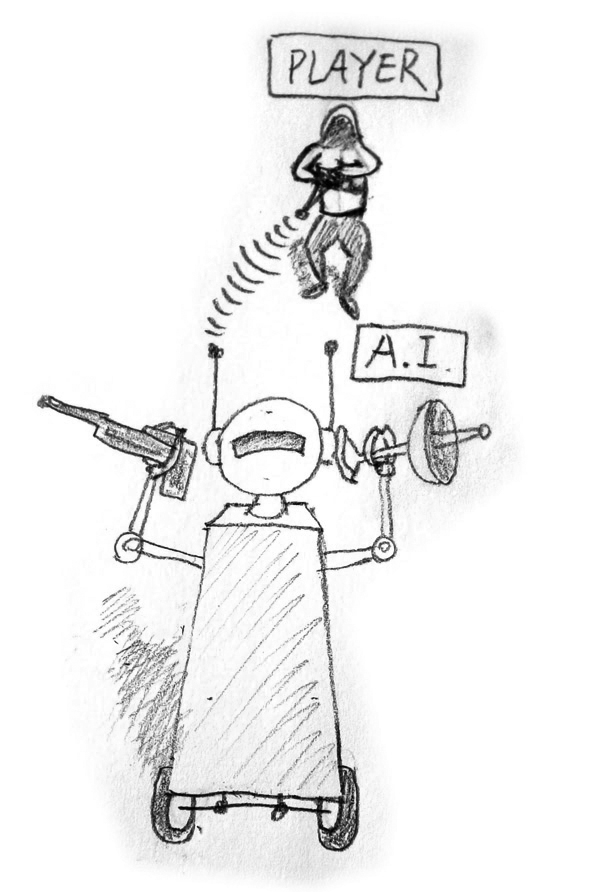
\includegraphics[scale=0.3]{design_draft_1.jpg}\\

Players provide A.I. controlling code to tell their A.I.s what to do. The game engine provides 3 sets of controlling APIs such as move, search, aim/fire. The difference between A.I. Craft and Robocode, however, besides being multiplayer and online, is mainly about players' ability to program.\\

To satisfy the goal of gamify learning, letting the players compete with each others on their ability to program is important. That is where the need for livecoding comes in. In the starting of a match, two players with their A.I. in ``null" state will be spawned into the game scene.\\ 

Players will submit their controlling code from there, thus they will have to take the code that is submitting by the opposite into consideration. For example, an experienced player will probably be submiting attacking code in the first place so that if the novice player is doing the same, they would got the lower hand. Therefore the novice player should consider to submit dodging code first.\\ 

Another major different from Robocode is to physically put the players into the arena. One of the purpose is to allow players to submit code to the A.I.s within a limited distance. This will give the players an immersive feeling when playing the game. Another purpose is to provide some new API calls such as follow(), so that the A.I. can follow the player's movement to avoid opposite attacks in the beginning. This ``following mode" provides great survivability for novice players even if they are facing an veteran. 



\section{Technical Details(Draft)}

\subsection{NodeJS}
``Node.js is a platform built on Chrome's JavaScript runtime for easily building fast, scalable network applications. Node.js uses an event-driven, non-blocking I/O model that makes it lightweight and efficient, perfect for data-intensive real-time applications that run across distributed devices."\cite{nodejs}\\

In other words, NodeJS is a browser javascript engine running on the serverside for serving network contents, similar to Perl/PHP/Ruby etc.. Since my players will be submitting javascript code, and the javascript code will be run on serverside in real time to control their A.I.s, choosing NodeJS seems obvious. NodeJS will be used to fulfill these features:\\
\\
1. Serving front end HTML/WebGL files\\
2. Connecting to database\\
3. Checking if user submitted code is secure\\
4. Executing user submitted code in real time\\
5. Executing and storing game logic in real time\\

\subsection{WebGL/HTML5}
WebGL is a software graphical library that extends the capability of the JavaScript programming language to allow it to generate interactive 3D graphics within any compatible web browser. \\

HTML is a language for structuring and presenting content for the World Wide Web. At version 5, HTML now provides a rich set of APIs such as socket communication, multi-threading and local storage, to enable rich interactive applications in browser.\\

Online game clients nowadays have three forms of distribution: Binary executable downloads, running in a browser plugin and running in a browser natively with no plugin required.\\ 

Performance wise, binary executable game clients are superior, since they often are making use of DirectX/OpenGL libraries and pre-compiled at run-time. However, its downside is platform dependent and users need to trust your binary code before they are willing to run it. Not being platform independent will greatly extend the development cycle, thus A.I. Craft will not be using this form of distribution.\\ 

Browser plugin games, on the other hand, such as flash games which require a plugin to run in browser, is now considered out-of-dated and unfashion after WebGL/HTML5 have been introduced. Because the trend of more devices will be supporting HTML5/WebGL and less devices will support flash and other web browser plugins, A.I. Craft will be using the third form if distribution: running in browsers natively.\\ 

Unfortunately, Microsoft internet exporleror has not provided support for WebGL and Socket communications, therefore IE users will not be supported by A.I. Craft. Firefox and Chrome users will be the targeted audience.\\


The animation and physical calculation of the game will be running in browser. Features included:\\
\\
1. Rendering the game scene, player A.I.s and other game objects\\
2. Calculating collision detections\\
3. Submitting players codes in real time\\
4. Preventing players from submitting pre-coded segments\\

\subsection{Database engine}
``A short definition of an RDBMS is: a DBMS(database management system) in which data is stored in tables and the relationships among the data are also stored in tables. The data can be accessed or reassembled in many different ways without having to change the table forms." -- Wikipedia\\

For A.I. Craft, the database will be served as a cloud storage for player information such as levels, currencies etc. RDBMS are not very useful for games because they cannot efficiently store heavily structured hierarchical data\cite{ari}.\\ 

A document-oriented database is a computer program designed for storing, retrieving, and managing document-oriented, or semi structured data, information. This kind of databases are much better for games, as they are more flexible in how they model data, while being more performant than relational databases\cite{michael10}. Therefore Document-oriented databases are my options. The current candidates are MangoDB, CouchDB and Redis.\\

\subsection{Software architecture}

``Prototype-based programming is a style of object-oriented programming in which classes are not present, and behavior reuse (known as inheritance in class-based languages) is performed via a process of cloning existing objects that serve as prototypes." -- Wikipedia\\

The whole game of A.I. Craft is based on Javascript, which is a prototype-based programming language. Here is a very basic layer of the game engine in Class Digram:\\

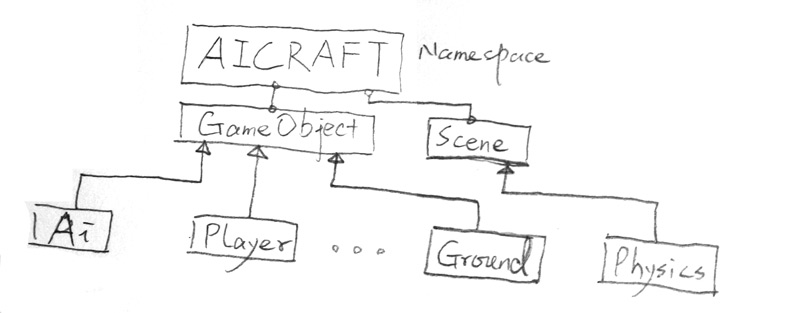
\includegraphics[scale=0.4]{uml.jpg}\\

The Scene class provides the game loop, thus there are varity of components for physics engine and graphic engine. The GameObject class is very interesting. All classes under GameObject tie to the game loop: they tell the game loop how much they weight, what models they will be using, what is the bounding box/octree they are binding to for collision dections, and the AI code that controls how they will react to various situtions etc.\\

The Ai Class, therefore, is the most interesting one. It is exposed to players to ``prototype" on its AI part. Here is a draft idea of what kind of code the players will be submitting:

\begin{verbatim}
AICRAFT.Ai.prototype.onScannedRobot(e) {
  this.fireAt(e.enemy.position);
 }
\end{verbatim}

Or:

\begin{verbatim}
myAi.__proto__.onScannedRobot(e) {
  this.fireAt(e.enemy.position);
 }
\end{verbatim}

Where AICRAFT.Ai is the ``Class", which really is the constructor function since every thing is Javascript is an object. And myAi is an instance.\\

Each code submitting would only allow one prototype in one function, thus forcing the player to ``livecode" their A.I., but not copying a big chunk of existed code which is equal to cheating.\\

By prototyping on the A.I. object, players therefore intractively improvise their A.I.s on the fly. And this is the core concept of the A.I. Craft project.\\

\begin{thebibliography}{9}

\bibitem{robocode01}
	Mathew Nelson, Flemming Larsen, IBM etc.\\
	\emph{Robocode}.\\
	\url{http://robocode.sourceforge.net}\\
	2001

\bibitem{noah2004}
	Noah Falstein,\\
	\emph{Natural Funativity}.\\
	\url{http://www.gamasutra.com/view/feature/2160/natural\_funativity.php}\\
	2004.

\bibitem{venkatesh2011}
	Venkatesh Rao,\\
	\emph{The Rise of Developeronomics}.\\
	\url{http://www.forbes.com/sites/venkateshrao/2011/12/05/the-rise-of-developeronomics/}\\
	2011.

\bibitem{robowiki1}
	\emph{Robot Anatomy}. \\
	\url{http://robowiki.net/wiki/Robocode/Robot\_Anatomy}\\
	2008.

\bibitem{nodejs}
	Ryan Dahl,\\
	\emph{NodeJS official site}.\\
	\url{http://www.nodejs.org}

\bibitem{ari}
	Ari Patrick,\\
	\emph{Why NoSQL databases are better for games}.\\
	\url{http://gamedev.stackexchange.com/questions/5316/nosql-is-it-a-valid-option-for-web-based-game}

\bibitem{michael10}
	Michael Kennedy,\\
	\emph{MongoDB vs. SQL Server 2008 Performance Showdown}.\\
	\url{http://www.michaelckennedy.net/blog/2010/04/29/MongoDBVsSQLServer2008PerformanceShowdown.aspx}\\
	2010

\end{thebibliography}

	

\end{document}

